%================================================================================
%== SETUP - CAN IGNORE
%================================================================================
\documentclass[10pt,letterpaper,subeqn]{beamer}
\setbeamertemplate{navigation symbols}{}
\usefonttheme{serif}
\usecolortheme{seahorse}
%\usecolortheme{orchid}



\usepackage[english]{babel}
\selectlanguage{english}
\usepackage{bm}
\usepackage{booktabs}
\usepackage{color}
\usepackage[update,prepend]{epstopdf}
\usepackage{framed}
\usepackage{fleqn}
\usepackage{graphics}
\usepackage{hyperref}
\usepackage[utf8]{inputenc}
\usepackage{setspace}
\usepackage{textcomp}
\usepackage{wrapfig}
\usepackage{multirow}
\usepackage{caption}
\usepackage{subcaption}
\setbeamertemplate{caption}[numbered]

\definecolor{bluegray}{rgb}{0.4, 0.6, 0.8}
\definecolor{babyblueeyes}{rgb}{0.63, 0.79, 0.95}
\definecolor{indigo}{rgb}{0.0, 0.25, 0.42}
\definecolor{navyblue}{rgb}{0.0, 0.0, 0.5}

%================================================================================
%== TITLE, NAMES, DATE
%================================================================================
\title{The Twin Instrument}
\subtitle{Mother's Health and the Quantity--Quality Trade-off}
\author{Sonia Bhalotra\inst{\dag} \and Damian Clarke\inst{\ddag}}
\institute{\inst{\dag} University of Essex \and \inst{\ddag} University of Oxford}
\date{August 2015}



\begin{document}


\begin{frame}
\titlepage
\end{frame}



%================================================================================
%== Slide 2: Twins: A Natural Experiment
%================================================================================

\section{Introduction}
\frame{\frametitle{This Talk}

\begin{enumerate}
\item \textbf{Twin births \emph{are not} exogenous}: even if twin conceptions are 
exogenous, taking twins to term depends on health stocks and behaviours of 
mothers during pregnancy \vspace{2mm}
\item We present the first evidence that this is a widespread phenomenon in rich 
and poor countries \vspace{2mm}
\item This results in \textbf{inconsistent estimates in studies using twins} as 
an instrument for fertility to estimate the Q--Q trade-off \vspace{2mm}
\item The IV bias is positive (OLS bias is negative). We show that bias-correction 
approaches produce stronger evidence of a trade-off \vspace{2mm}
\item  Previous ignorance of this bias contributes to explaining the tendency for 
recent studies to reject the presence of a Q--Q tradeoff (Angrist et al.\ 2010, 
Black et al.\ 2005)
\end{enumerate}
}

\frame{
\begin{center}
\Large \textbf{Introduction}
\end{center}
}

\frame{\frametitle{Twins -- A Natural Experiment (1)}
\begin{itemize}
\item A vast literature in economics, behavioural genetics and psychology relies 
upon the premise that twin births occur as an act of nature -- and are allocated 
randomly across families.\\ \vspace{5mm}
\item A twin birth generates a natural experiment. 
\begin{itemize}
\item It allows us to compare families that unexpectedly have an additional child 
because they have a twin birth with families who have the same number of birth 
events but only singleton births. \\ \vspace{5mm}
\end {itemize} 
\item This is useful when one is interested in identifying causal effects of 
fertility (number of children) on investments in child quality (e.g. education), 
or on mothers' workforce participation.
\end{itemize}
}

\frame{\frametitle{Twins -- A Natural Experiment (2)}
\begin{itemize}
\item The `identification' challenge is to isolate causal effects of fertility 
from the mother's preferences and characteristics: 
\begin{itemize}
\item Women who prefer to have more children may be women who chose to invest 
less in their own education and who may prefer to invest less in their children, 
or prefer not to work. \\ \vspace{5mm}
\end{itemize} 
\item If a twin birth is a random event it does the trick because it is by 
definition detached from the mother's characteristics. It simply \emph{drops} 
an additional child on some families and not on others. \\ \vspace{5mm}
\item Twins are not as rare as we may think: 1 in 80 live births, so 1 in 40 
babies is a twin.
\end{itemize}
}

\begin{frame}[label=FS1]
\frametitle{Twins Shift Distribution of Family Size}
\begin{figure}[htpb!]
\centering
  %\caption{Total births by Family Type}
  %\label{TWINfig:famsize}
  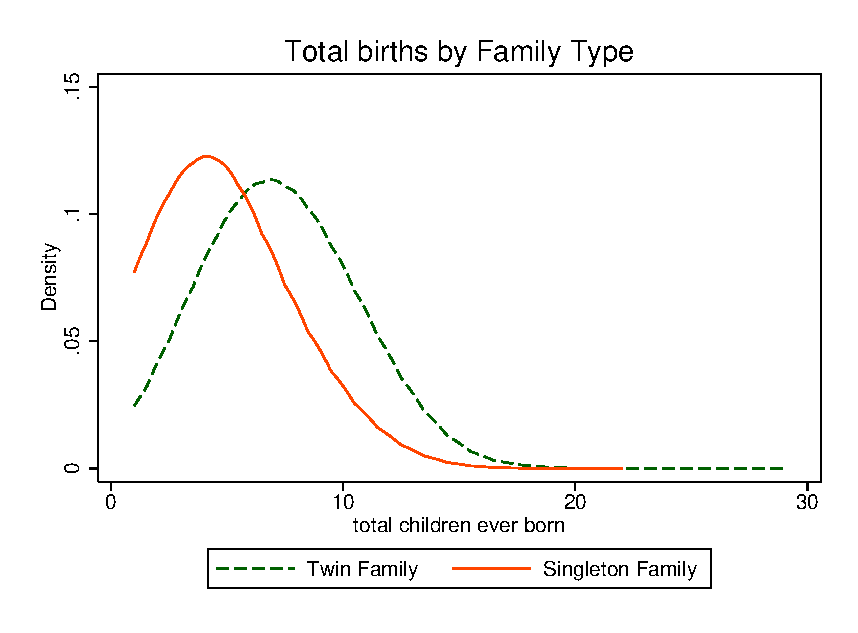
\includegraphics[scale=0.75]{./figures/famsize.eps}
\end{figure}
\hyperlink{Fstage}{\beamergotobutton{Regression}}
\end{frame}

%================================================================================
%== Slide 2: Twin Births Are Not Random
%================================================================================

\frame{\frametitle{Twin Births Are Not Random}
\begin{itemize}
\item We argue that even if twin conceptions are `random', twin births are not 
because taking twins to term depends on health stocks and behaviours of mothers 
during pregnancy.
\item The natural experiment breaks down and studies relying upon it produces 
biased estimates.\\ \vspace{5mm}
\item We present the first evidence that this is a widespread phenomenon in rich 
and poor countries
\item In poor countries, many women are severely under-nourished and may not be 
fit enough to carry twin conceptions to birth. 
\item In richer countries, many women engage in risky behaviours and/or experience 
medical problems in pregnancy.
\end{itemize}
}

\begin{frame}[label=mech]
\frametitle{Mechanisms}
\begin{itemize}

\item There is some medical evidence to support our contention: FSH is associated with the risk of dizygotic twins and is more prevalent among heavier and taller women: Hall (2003). \\ \vspace{3mm}
\item The mechanism is selective fetal death. 
\begin{itemize}
\item Twin conceptions are more demanding of maternal resources and hence more likely to suffer miscarriage or stillbirth.
\item It is estimated that 1 in 8 twin conceptions results in a live birth. The spontaneous abortion rate is three times that for singletons (Boklage 1990). \\ \vspace{3mm}
\end{itemize}
\item Hard to find data on twin conceptions and on miscarriage. We found relevant data from \hyperlink{TwinDeathNepal}{\textcolor{blue}{USA}} and \hyperlink{TwinDeathSpain}{\textcolor{blue}{Spain}} which establish that:
\begin{enumerate}
\item[(i)] Miscarriage is more frequent among less healthy women (health indicated by under-weight, short, hypertension, etc.)
\item[(ii)] Miscarriage is more frequent among twins
\item[(iii)] and is more frequent among less healthy women carrying twins
\end{enumerate}
\end{itemize}
\end{frame}





%================================================================================
%== Slide 3: The Quantity-Quality Tradeoff
%================================================================================
\frame{\frametitle{The Quantity--Quality Trade-off}
\begin{itemize}

\item To illustrate the substantive implications of the problem and its empirical significance, we re-consider the body of work in which economists leverage the occurrence of twin births to estimate causal effects of fertility on child education and other measurable `quality' variables like child health. \vspace{3mm}
\item Evidence from cross-sectional data within and across regions suggests that children from larger families have weaker educational outcomes, e.g. Hanushek (1992), Blake (1989). 
\end{itemize}
}

\begin{frame}[label=Macro]
\frametitle{Trends in Education, Fertility, Fertility Control}
\begin{figure}[htpb!]
\centering
\begin{subfigure}{.5\textwidth}
  \centering
  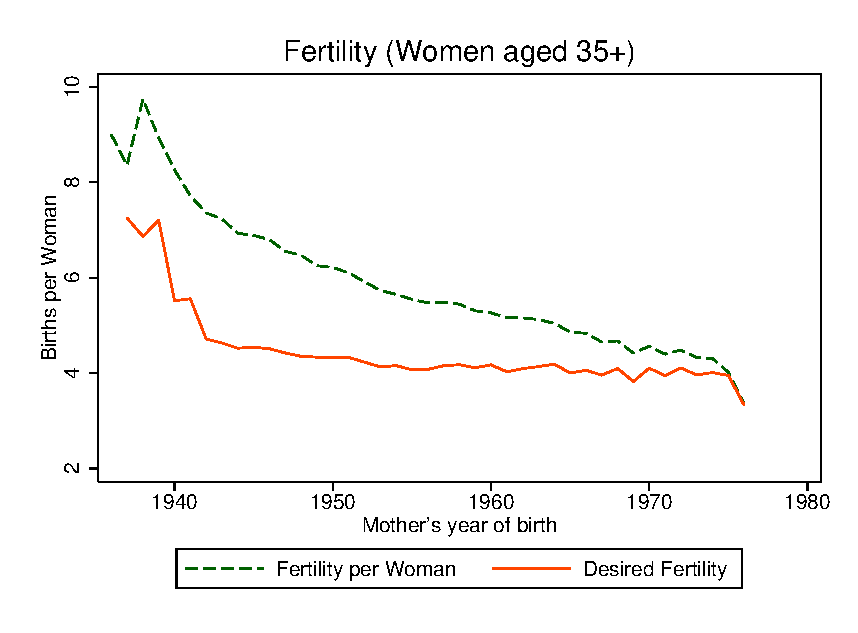
\includegraphics[scale=0.39]{./figures/ferttrend_35_all.eps}
  \caption{Trends in Fertility}
  \label{TWINfig:fertrend}
\end{subfigure}%
\begin{subfigure}{.5\textwidth}
  \centering
  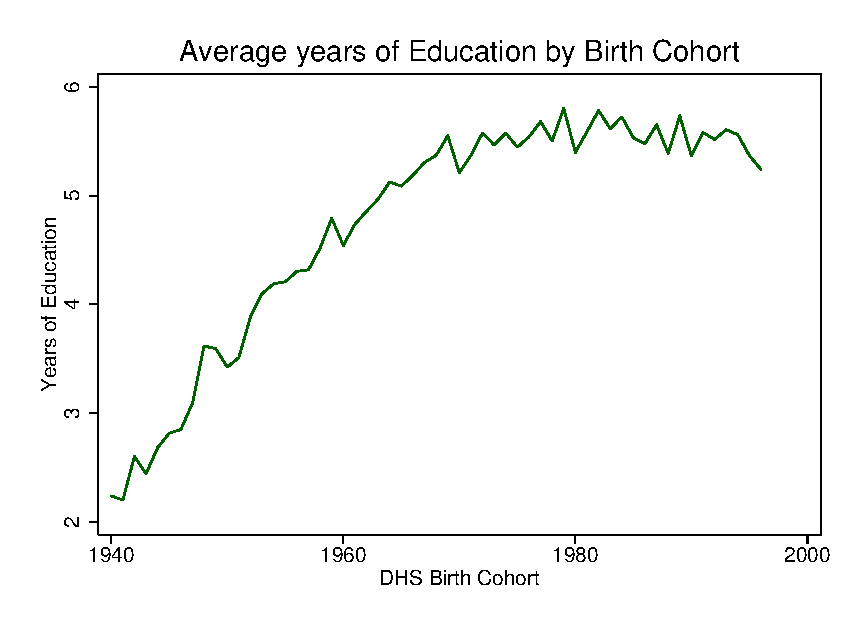
\includegraphics[scale=0.39]{./figures/eductrend_all.eps}
  \caption{Trend in Education}
  \label{TWINfig:eductrend}
\end{subfigure}
\caption{Education and Fertility}
\label{TWINfig:trends}
\end{figure}
\footnotesize{Note to figures: Cohorts are made up of all individuals 
from the DHS who are over 35 years (for fertility), and over 15 years (for education).  
The sample is restricted to those who have approximately completed fertility 
and education respectively.}
\end{frame}



\frame{\frametitle{The Quantity--Quality Trade-off (continued)}
\begin{itemize}
\item In the time series, fertility has tended to decline while investments in education increase, e.g. Galor 2012. \vspace{3mm}
\begin{itemize}
\item This empirical regularity has been attributed to a quantity--quality (Q--Q) trade-off in parental investments: Becker and Lewis 1973, Becker and Tomes 1976. A `pillar' in theories of the economics of the family. 
\item It has shaped economic thinking and, also, aggressive fertility-control policies.
\end{itemize}
\item However recent studies reject the presence of a Q--Q tradeoff (Angrist et al.\ 2010, Black et al.\ 2005) \vspace{3mm}
\item We show that a trade-off emerges upon (partial) correction for the twin-bias: substantive relevance of our critique 
\end{itemize}
}



\frame{
\begin{center}
\Large \textbf{Empirical Framework}
\end{center}
}



\frame{\frametitle{IV Procedure}
OLS fails to recover consistent estimates of the Q--Q trade-off (endogeneity, multiplicative entry of Q--Q).  Often, use IV:
\vspace{6mm}
\begin{equation}
\label{TWINeqn:secondstage}
educ_{ij}=\beta_0+\beta_1 fert_{j} + \bm{X}\bm{\beta}_2+u_{ij}.
\end{equation}
\begin{equation}
\label{TWINeqn:firststage}
fert_{j}=\alpha_0+\alpha_1 twins_{j}+\bm{X}\bm{\alpha}_2+\nu_{j},
\end{equation}
\vspace{2mm}
And so assuming:
\[
\mathbb{E}[fert_j\cdot u_{ij}] \neq 0, \ \mathbb{E}[twins_j\cdot u_{ij}] = 0
\]
\vspace{6mm}
\begin{itemize}
\item Previous studies assume twin incidence is a valid instrument.
\item A key concern is whether IV estimates are precise enough to be informative (and distinguishable from OLS estimates): Angrist et al.\ (2010).
\end{itemize}
}

\frame{\frametitle{Investigating Exogeneity of Twins (I)}
\begin{equation}
\label{TWINeqn:twinreg}
P(twin_{j})=\gamma_0 + \bm{X}\bm{\gamma}_1 + \bm{S}\bm{\gamma}_2
                  + \bm{H}\bm{\gamma}_3 + \varepsilon_{j}.
\end{equation}
\begin{itemize}
\item $\bm{X}, \bm{S}$ and $\bm{H}$ are mother characteristics potentially correlated with child quality: age, wealth, education, height, BMI during pregnancy, antenatal care availability, smoking/drinking/drugs during pregnancy.
\item If twin birth is a random event $\bm{\gamma_1}=\bm{\gamma_2}=\bm{\gamma_3}=0$
\item Can typically condition on only a subset of predictors $X$
\item Equivalent: test of balance of characteristics between mothers who have twins (quasi-treatment) and mothers who do not (quasi-control)
\end{itemize}
}

\frame{\frametitle{Investigating Exogeneity of Twins (II)}
Examine whether women who have twins are healthier before twins occurr:
\vspace{2mm}
\[Quality_{t-k}=\alpha twins_{t}+\bm{X}\delta + \varepsilon \]
\vspace{5mm}
\begin{itemize}
\item Compare child quality in families with and without twins at parity $p$ for children born at earlier parities. 
\item But use a measure of quality (investment) that is necessarily determined before twins occur: infant mortality.
\item If twins occur randomly, $\alpha=0$.  If positively selected, $\alpha<0$.
\end{itemize}
}



\frame{\frametitle{How We Investigate Inconsistency in Estimators That Assume Twins Are Random}
\begin{itemize}
\item The bias could be corrected if all relevant aspects of maternal health were fully measurable and observable. 
\item But maternal health and pregnancy behaviours are multidimensional and partially unobserved.  
\item In order to put limits on the inconsistency in existing studies, we use a number of partial
identification and bounding techniques:
\end{itemize}
\vspace{5mm}
\begin{enumerate}
\item[1:] Introduce available (partial) controls for maternal health, estimating bounds on the parameter of interest
\begin{itemize}
\item Bound between (upward biased) OLS and (downward biased) IV
\end{itemize} \vspace{5mm}
\item[2:] Ask how `non-random' twins need to be for the true effect to be statistically different from zero. 
\begin{itemize}
\item Estimate bounds this way: Conley et al.\ (2012).
\end{itemize}
\end{enumerate}
}

\frame{\frametitle{Twin Endogeneity and IV Inconsistency}
Assuming additive separability of $u_{ij}$: $u_{ij}=u_{ij}^S+u_{ij}^H+u_{ij}^*$.  The typical IV estimate is 
then the population value, plus (unobserved) error components:
\[
\hat\beta_1^{IV} = \beta_1 + P\lim \frac{1}{N}\sum_{j=1}^{N}twin_j(u^S_{ij} + u^H_{ij} + u^*_{ij})
\]

\vspace{6mm}
We can remove certain observed variables from the error term.  By including elements $S$ and $H$ as additional controls in $\bm{X}$, the IV estimate becomes:
\[
\hat\beta_1^{IV,S+H} = \beta_1 + P\lim \frac{1}{N}\sum_{j=1}^Ntwin_ju^*_{ij},
\]
\vspace{3mm}
where it is likely that $\hat\beta_1^{IV}>\hat\beta_1^{IV,H}>\hat\beta_1^{IV,S+H}>\beta_1.$
}

\frame{\frametitle{Twin Endogeneity and IV Inconsistency}
\begin{center}
\[
\hspace{2cm} \hat\beta_1^{IV}>\hat\beta_1^{IV,H}>\hat\beta_1^{IV,S+H}>\beta_1.
\]
\end{center}
\vspace{6mm}
\begin{spacing}{1.2}
Maternal health and pregnancy behaviours are multidimensional and partially unobserved.  In order
to put limits on the inconsistency $\hat\beta_1^{IV,S+H}>\beta_1$, we use a number of partial
identification and bounds techniques
\end{spacing}
\vspace{2mm}
\begin{itemize}
\item Bound between (upward biased) OLS and (downward biased) IV
\item Combine OLS with Altonji-Taber, and Oster bounds
\item Combine IV with Conley et al bounds (similar to Rosen and Nevo)
\end{itemize}
}



%================================================================================
%== Slide 12: Data
%================================================================================

\frame{
\begin{center}
\Large \textbf{Data}
\end{center}
}

\section{Data}
\frame{\frametitle{Data}
\begin{enumerate}
\item Developing Countries
\begin{itemize}
\item Comparable cross-country micro-data for developing countries
\item Surveys conducted 1991-2013: sample of $\sim$3 million children born in 
68 countries. Birth cohorts 1971-2012
\item Large sample useful given twins are rare (sample mean 1.85\%) \\ \vspace{4mm}
\end{itemize}
\item USA
\begin{itemize}
\item American National Health Interview Surveys conducted 2004-2014 \\ \vspace{4mm}
\end{itemize}
\item Microdata from many other countries\ldots
\begin{itemize}
\item Administrative birth registries and surveys in the UK, Scotland, Spain, Chile, 
Brazil, Sweden.
\end{itemize}
\end{enumerate}
}

\begin{frame}[label=sumStats]
\begin{table}[htpb!]\caption{Summary Statistics} 
\label{TWINtab:sumstats}\begin{center}\scalebox{0.6}{\begin{tabular}{lccccc}
\toprule \toprule 
&\multicolumn{2}{c}{Low Income}&\multicolumn{2}{c}{Middle Income}\\ 
\cmidrule(r){2-3} \cmidrule(r){4-5}
& Single & Twins & Single & Twins & All \\ \midrule 
\textsc{Fertility} & & & & & \\ 
Fertility&3.670&6.093&3.348&5.425&3.609\\
&(2.365)&(2.582)&(2.272)&(2.609)&(2.372)\\
Desired Family Size&4.182&5.296&3.340&4.128&3.892\\
&(2.500)&(2.832)&(2.083)&(2.498)&(2.403)\\
Fraction Twin & \multicolumn{2}{c}{  0.0194}& \multicolumn{2}{c}{  0.0173 } &  0.0185\\
& \multicolumn{2}{c}{(0.1379)}& \multicolumn{2}{c}{(0.1306)} & (0.1348)\\
\textsc{Health of Mother}&&&&&\\ 
Height&155.6&157.7&155.6&157.2&155.7\\
&(7.084)&(6.987)&(6.956)&(6.957)&(7.042)\\
BMI&21.89&22.47&25.83&26.50&23.38\\
&(3.983)&(4.098)&(5.066)&(5.437)&(4.822)\\
Pr(BMI)$<$18.5&0.172&0.123&0.0344&0.0276&0.119\\
&(0.377)&(0.328)&(0.182)&(0.164)&(0.324)\\
\textsc{Children's Outcomes}&&&&&\\ Education (Years)
&3.695&3.212&5.438&4.999&4.465\\
&(3.581)&(3.270)&(3.859)&(3.734)&(3.805)\\
Education (Z-Score)&-0.00869&-0.0130&0.0121&-0.0366&0.000177\\
&(1.001)&(0.961)&(0.998)&(0.987)&(1.000)\\
\midrule
Number of Countries &42&42&34&34&68 \\
Number of Mothers &491,905 &7,457 &297,413 &4,317 & 850,032 \\
Number of Children (Education) &1,176,513 &25,003 &714,751 &14,333 & 1,930,600 \\
Number of Children (Ever Born) &1,716,247 &43,866 &940,204 &21,302 & 2,721,619 \\
\midrule
\multicolumn{6}{p{13.8cm}}{\begin{footnotesize}\textsc{Notes:} Group means (sd).\end{footnotesize}} \\ \bottomrule \end{tabular}}\end{center}\end{table}

\hyperlink{sumStatsN}{\beamergotobutton{NHIS Summary Statistics}}
\end{frame}

\frame{\frametitle{Data and Context}
\begin{itemize}
\item Effects of twins at parity $k$ on outcomes for births $k-1$ and before 
(as in Black et al. 2005). 
\begin{itemize}
\item Predictions are for infra-marginal children.
\end{itemize}
\item Nomenclature: ``2+ sample'': Firstborn subjects in families with at least two births (allowing that a birth may be twin). 
\begin{itemize}
\item Instrument with twins at second birth
\end{itemize}
\item ``3+ sample'': First and second born subjects in families with at least three births 
\begin{itemize}
\item Instrument with twins at third birth
\end{itemize}
\item And simiarly for 4+.  Twin subjects are generally dropped.
\end{itemize}
}

\frame{\frametitle{Data and Context}
\begin{itemize}
\item By restricting to families with at least $k$ births on average we ensure that preferences over family size are the same in the families with twins at the $k^{th}$ birth and those with singleton births
\item By restricting the sample to children born before birth $k$, we avoid selection problems that arise because families who choose to have another child after a twin birth may differ from families who choose to have another child after a singleton birth.
\end{itemize}
}


\section{Results}
\frame{
\begin{center}
\Large \textbf{Results}
\end{center}
}

\frame{\frametitle{Results}
\begin{itemize}
\item \textbf{Twin `Endogeneity'}
\item The Q--Q Trade-off
\item Bounding Q--Q Estimates
\end{itemize}
}

\subsection{Twin Births Are Correlated With Mother Characteristics}
\frame{\frametitle{Mother's Health}
\begin{itemize}
\item No previous evidence (or discussion) of maternal health being a predictor of twin births.
\item But, recognised that maternal health and behaviours affects a large number of other birth and longer term outcomes (Mazumder and Seeskin, 2014; Black et al.\ 2014;  Bhalotra and Rawlings 2013; Almond et al.\ 2011; Barker 1995).
\item And evidence from medical literature (Li et al.\ 2003, Hall 2003) that Pr(twinning) increases with age, weight and height (mediated by follicle stimulating hormone) 
\item We compile many datasets and measures of mother health stocks and behaviours preceding births
\end{itemize}
}


\frame{
\begin{figure}[htpb!]
\centering
  \caption{Height as a Proxy for Health and Twinning}
  \label{TWINfig:height}
  \includegraphics[scale=0.75]{./figures/height_country.eps}
\end{figure}
}


\frame{
\vspace{5mm}
\begin{landscape}\begin{table}[htpb!] 
\caption{Probability of Giving Birth to Twins} \label{TWINtab:twinreg1} 
\begin{center}\begin{tabular}{lcccccc} \toprule \toprule 
&(1)&(2)&(3)&(4)&(5)&(6)\\
Twin*100&All&\multicolumn{2}{c}{Income}&\multicolumn{2}{c}{Time}&Prenatal\\
 \cmidrule(r){3-4} \cmidrule(r){5-6} 
&&Low inc&Middle inc&1990-2013&1972-1989&\\\midrule
\begin{footnotesize}\end{footnotesize}&\begin{footnotesize}\end{footnotesize}&\begin{footnotesize}\end{footnotesize}&\begin{footnotesize}\end{footnotesize}&\begin{footnotesize}\end{footnotesize}&\begin{footnotesize}\end{footnotesize}&\begin{footnotesize}\end{footnotesize}\\
Age&0.596***&0.615***&0.554***&0.647***&0.326***&0.631***\\
&(0.029)&(0.036)&(0.050)&(0.033)&(0.075)&(0.040)\\
Age Squared&-0.008***&-0.008***&-0.008***&-0.009***&-0.003**&-0.009***\\
&(0.001)&(0.001)&(0.001)&(0.001)&(0.001)&(0.001)\\
Age First Birth&-0.053***&-0.093***&0.004&-0.052***&-0.056***&-0.041***\\
&(0.009)&(0.012)&(0.014)&(0.010)&(0.019)&(0.013)\\
Education (years)&0.042**&0.089***&-0.005&0.048**&0.022&-0.068**\\
&(0.017)&(0.022)&(0.029)&(0.020)&(0.034)&(0.028)\\
Education squared&-0.002&-0.006***&0.001&-0.002&0.000&0.003\\
&(0.001)&(0.002)&(0.002)&(0.002)&(0.003)&(0.002)\\
Height&0.058***&0.057***&0.059***&0.062***&0.042***&0.058***\\
&(0.004)&(0.005)&(0.007)&(0.005)&(0.008)&(0.007)\\
BMI&0.048***&0.063***&0.039***&0.046***&0.055***&0.044***\\
&(0.006)&(0.009)&(0.009)&(0.007)&(0.011)&(0.011)\\
Prenatal (Doctor)&&&&&&0.906***\\
&&&&&&(0.128)\\
Prenatal (Nurse)&&&&&&0.067\\
&&&&&&(0.108)\\
Prenatal (None)&&&&&&-0.497***\\
&&&&&&(0.132)\\
&&&&&&\\R-squared&0.01&0.01&0.01&0.01&0.01&0.01\\
Observations &1930653&1201555&729098&1524947&405706&615935\\
\hline\hline\multicolumn{7}{p{14.3cm}}{\begin{footnotesize}\textsc{Notes:} All specifications include a full set of year of birth and  country dummies, and are estimated as linear probability models.  Twin is multiplied by 100 for presentation.  Height is measured in cm  and BMI is weight in kg divided by height in metres squared. l  Prenatal care variables are only recoreded for recent births.  As  such, column (6) is estimated only for that subset of births where  these observations are made.
$^{*}$p$<$0.1; $^{**}$p$<$0.05; $^{***}$p$<$0.01
 \end{footnotesize}}\\ \hline \normalsize \end{tabular}\end{center}\end{table}\end{landscape} 

}


%================================================================================
%== Slide 17: Effect Sizes
%================================================================================
\begin{frame}[label=robust]
\frametitle{Effect Sizes}
Substantial marginal effects of observed indicators of mother’s health on the probability of twin birth (mean$\approx$2\%)
\vspace{6mm}
\begin{itemize}
\item $\Delta^+$ 1 s.d.\ height of mother $\rightarrow$ $\Delta^+$ twin 0.44\% (22\% of mean)
\item $\Delta^+$ 1 s.d.\ BMI of mother \ \ $\rightarrow$ $\Delta^+$ twin 0.20\% (10\% of mean)
\item Potential bias on account of selection on maternal survival. 
\item We (over-)correct for this and establish that selection does not drive our findings. \hyperlink{MMRselec}{\beamergotobutton{Procedure}}
\end{itemize}
\end{frame}

\begin{frame}[label=c]
\frametitle{Is This an Artifact of DHS Data?}
\begin{itemize}
\item We have compiled evidence using a number of surveys and administrative data sets:
  \begin{itemize}
  \item \hyperlink{Chile}{\textcolor{blue}{Chile}}
  \item \hyperlink{UK}{\textcolor{blue}{UK}}
  \item \hyperlink{USA1}{\textcolor{blue}{USA}} (National Vital Statistics System)
  \item \hyperlink{USA2}{\textcolor{blue}{USA}} (National Health Surveys)
  \item \hyperlink{Scotland}{\textcolor{blue}{Scotland}}$^*$
  \item \hyperlink{Spain1}{\textcolor{blue}{Spain}}$^*$ (Birth Registry)
  \item \hyperlink{Spain2}{\textcolor{blue}{Spain}}$^*$ (terror shock from Quintana-Domeque and R\'odenas)
  \item \hyperlink{Brazil}{\textcolor{blue}{Brazil}}$^*$
  \item \hyperlink{Sweden}{\textcolor{blue}{Sweden}}$^*$
 \end{itemize}
\item Depending upon data availability we include health stocks, behaviour
\item This is not restricted to poor countries.
\item Mechanism?  \hyperlink{TwinDeath}{\textcolor{blue}{Evidence}} that twins are more likely to die in utero when health stocks are low.
\end{itemize}
\end{frame}

\begin{frame}[label=USA1]
\begin{table}[htpb!]
\caption{United States Birth Registry (Administrative 2003-2012)}
\begin{center}
\scalebox{0.54}{
\begin{tabular}{lcccc} \hline
 & (1) & (2) & (3) & (4) \\
VARIABLES & twin100 & twin100 & twin100 & twin100 \\ \hline
\vspace{4pt} & \begin{footnotesize}\end{footnotesize} & \begin{footnotesize}\end{footnotesize} & \begin{footnotesize}\end{footnotesize} & \begin{footnotesize}\end{footnotesize} \\
africanAmerican & 0.554*** & 0.437*** & 0.437*** & 0.331*** \\
\vspace{4pt} & \begin{footnotesize}(0.00911)\end{footnotesize} & \begin{footnotesize}(0.0142)\end{footnotesize} & \begin{footnotesize}(0.0142)\end{footnotesize} & \begin{footnotesize}(0.0143)\end{footnotesize} \\
otherRace & 0.0433*** & 0.135*** & 0.135*** & -0.680*** \\
\vspace{4pt} & \begin{footnotesize}(0.00886)\end{footnotesize} & \begin{footnotesize}(0.0148)\end{footnotesize} & \begin{footnotesize}(0.0148)\end{footnotesize} & \begin{footnotesize}(0.0200)\end{footnotesize} \\
meducSecondary & 0.00124 & 0.0124 & 0.0124 & 0.810*** \\
\vspace{4pt} & \begin{footnotesize}(0.00881)\end{footnotesize} & \begin{footnotesize}(0.0159)\end{footnotesize} & \begin{footnotesize}(0.0159)\end{footnotesize} & \begin{footnotesize}(0.0203)\end{footnotesize} \\
meducTertiary & 1.124*** & 1.110*** & 1.110*** & 2.063*** \\
\vspace{4pt} & \begin{footnotesize}(0.00930)\end{footnotesize} & \begin{footnotesize}(0.0158)\end{footnotesize} & \begin{footnotesize}(0.0158)\end{footnotesize} & \begin{footnotesize}(0.0209)\end{footnotesize} \\
tobaccoUse & -0.327*** & -0.424*** & -0.424*** & -0.422*** \\
\vspace{4pt} & \begin{footnotesize}(0.0126)\end{footnotesize} & \begin{footnotesize}(0.0181)\end{footnotesize} & \begin{footnotesize}(0.0181)\end{footnotesize} & \begin{footnotesize}(0.0182)\end{footnotesize} \\
alcoholUse &  & -1.233*** & -1.233*** & -1.182*** \\
\vspace{4pt} & \begin{footnotesize}\end{footnotesize} & \begin{footnotesize}(0.0648)\end{footnotesize} & \begin{footnotesize}(0.0648)\end{footnotesize} & \begin{footnotesize}(0.0651)\end{footnotesize} \\
anemia &  &  &  & -1.349*** \\
\vspace{4pt} & \begin{footnotesize}\end{footnotesize} & \begin{footnotesize}\end{footnotesize} & \begin{footnotesize}\end{footnotesize} & \begin{footnotesize}(0.0335)\end{footnotesize} \\
diabetes &  &  &  & -0.408*** \\
\vspace{4pt} & \begin{footnotesize}\end{footnotesize} & \begin{footnotesize}\end{footnotesize} & \begin{footnotesize}\end{footnotesize} & \begin{footnotesize}(0.0280)\end{footnotesize} \\
chyper &  &  &  & -0.883*** \\
\vspace{4pt} & \begin{footnotesize}\end{footnotesize} & \begin{footnotesize}\end{footnotesize} & \begin{footnotesize}\end{footnotesize} & \begin{footnotesize}(0.0528)\end{footnotesize} \\
phyper &  &  &  & -4.128*** \\
\vspace{4pt} & \begin{footnotesize}\end{footnotesize} & \begin{footnotesize}\end{footnotesize} & \begin{footnotesize}\end{footnotesize} & \begin{footnotesize}(0.0267)\end{footnotesize} \\
eclamp &  &  &  & -5.686*** \\
\vspace{4pt} & \begin{footnotesize}\end{footnotesize} & \begin{footnotesize}\end{footnotesize} & \begin{footnotesize}\end{footnotesize} & \begin{footnotesize}(0.0896)\end{footnotesize} \\
Constant & 5.461*** & 5.326*** & 5.326*** & 32.75*** \\
 & \begin{footnotesize}(0.0525)\end{footnotesize} & \begin{footnotesize}(0.0806)\end{footnotesize} & \begin{footnotesize}(0.0806)\end{footnotesize} & \begin{footnotesize}(0.293)\end{footnotesize} \\
\vspace{4pt} & \begin{footnotesize}\end{footnotesize} & \begin{footnotesize}\end{footnotesize} & \begin{footnotesize}\end{footnotesize} & \begin{footnotesize}\end{footnotesize} \\
Observations & 38,910,055 & 16,605,619 & 16,605,619 & 12,219,256 \\
 $R^2$ & 0.008 & 0.008 & 0.008 & 0.012 \\ \hline
\multicolumn{5}{c}{\begin{footnotesize} Standard errors in parentheses\end{footnotesize}} \\
\multicolumn{5}{c}{\begin{footnotesize} *** p$<$0.01, ** p$<$0.05, * p$<$0.1\end{footnotesize}} \\
\end{tabular}}
\end{center}
\end{table}

\end{frame}

\begin{frame}[label=Chile]
\input{./tables/ChileTwin.tex}
\end{frame}

\begin{frame}[label=Spain2]
%\begin{figure}
%\caption{Twin Births and Stress (Quintana-Domeque and R\'odenas)}
\input{./tables/Stress.tex}
\end{frame}

\begin{frame}[label=Sweden]
\input{./tables/SwedenTwin2.tex}
\end{frame}

\begin{frame}[label=USA2]
\begin{table}[htpb]
\caption{Probability of Giving Births to Twins (NHIS, USA)}
\begin{center}
\scalebox{0.64}{
\begin{tabular}{lcc} \toprule
&(1)&(2) \\
VARIABLES&Twin$\times$100&Twin$\times$100 \\ \midrule
&& \\
Mother's Height&0.0416**&0.0406** \\
&(0.0201)&(0.0201) \\
Mother's Education&0.0084&0.0033 \\
&(0.0162)&(0.0164) \\
Smokes (pre-Pregnancy)&-0.119&-0.0983 \\
&(0.115)&(0.116) \\
Mother's Age&0.0121&0.0108 \\
&(0.0446)&(0.0446) \\
Mother's Age$^2$ &-0.0008&-0.0008 \\
&(0.0006)&(0.0006) \\
Age First Birth &0.166***&0.164*** \\
&(0.0135)&(0.0136) \\
BMI &0.0123***&0.0130*** \\
&(0.0034)&(0.0034) \\
Mother Good Health&&0.203* \\
&&(0.116) \\
Mother Poor Health&&-0.00284 \\
&&(0.189) \\
Constant&-4.091***&-4.101*** \\
&(1.542)&(1.543) \\
&& \\
Observations&105,879&105,879 \\
R-squared&0.004&0.004 \\ \midrule
%\multicolumn{3}{ p{5cm} }{\begin{footnotesize}\textsc{Notes:} Standard errors in parentheses. *** p$<$0.01; ** p$<$0.05; * p$<$0.1\end{footnotesize}}\bottomrule
\end{tabular}}
\end{center}
\end{table}

\end{frame}

\begin{frame}[label=Scotland]
\input{./tables/ScotlandTwin.tex}
\end{frame}


\frame{\frametitle{Second Test of Exogeneity of Twins: Are mothers who produce twins healthier ex ante?}
\begin{itemize}
\item Comparison of child outcome determined before twins arise across families who do and do not subsequently have a twin birth
\item Results indicate that twin births occur in families with a tendency towards lower infant morality, possibly healthier (or better-off) families.
\end{itemize}
\begin{table}[htpb!]\caption{IMR Test} 
\label{TWINtab:IMR}\vspace{-5mm}\begin{center}\begin{tabular}{lccc}
\toprule \toprule 
\textsc{IMR}& Base & +S\&H & Observations \\ \midrule 
\begin{footnotesize}\end{footnotesize}& 
\begin{footnotesize}\end{footnotesize}& 
\begin{footnotesize}\end{footnotesize}& 
\begin{footnotesize}\end{footnotesize}\\ 
Treated (2+)&-1.396**&-1.402**&337378\\
&(0.639)&(0.638)&\\
Treated (3+)\hspace{5mm}&-1.565***&-1.570***&455372\\
&(0.362)&(0.363)&\\
Treated (4+)&-0.634***&-0.620***&443165\\
&(0.066)&(0.066)&\\
Treated (5+)&-0.423***&-0.412***&382405\\
&(0.139)&(0.139)&\\
\midrule\multicolumn{4}{p{7cm}}{\begin{footnotesize}\textsc{Notes:} $^{*}$p$<$0.1; $^{**}$p$<$0.05; $^{***}$p$<$0.01 
\end{footnotesize}} \\ \bottomrule 
\end{tabular}\end{center}\end{table}
}

\frame{\frametitle{Test 3 (Suggestive): Healthier Cohorts $\rightarrow$ More Twins}
\begin{figure}[htpb!]
\centering
  \caption{Proportion of Twins of All Births (USA)}
  \label{TWINfig:UStwin}
  \includegraphics[scale=0.72]{./figures/USTwinFLE.eps}
\end{figure}
}

\begin{frame}[label=mechan]
\frametitle{Mechanism}
\begin{itemize}
\item Healthier women appear to be more likely to take twins to term 
\emph{conditional} on conceiving twins
\item In \hyperlink{USA3}{\textcolor{blue}{USA}} and \hyperlink{Spain3}{\textcolor{blue}{Spain}}:
\begin{itemize}
\item Unhealthy women are more likely to miscarry
\item Twins are more likely to miscarry
\item Unhealthy women with twins are more likely to miscarry than healthy women with twins
\end{itemize}
\item We show that this is not driven (entirely) by \hyperlink{surv}{\textcolor{blue}{selective maternal death}}
\end{itemize}
\end{frame}
%================================================================================
%== Slide 21: OLS and IV Estimates
%================================================================================
\frame{\frametitle{Results}
\begin{itemize}
\item Twin `Endogeneity'
\item \textbf{The Q--Q Trade-off}
\item Bounding Q--Q Estimates
\end{itemize}
}


\subsection{OLS and IV Estimates}
\frame{\frametitle{OLS and IV Estimates}
\begin{itemize}
\item OLS \emph{over}-estimates the trade-off because fertility is negatively correlated with child education.
\item To address this, fertility is instrumented with twin-birth widespread 
\item IV will \emph{under}-estimate the trade-off if twin-birth is non-random (because mothers who invest in their health are mothers who invest in children). 
\item Demonstrate both OLS and IV bias by conditioning on observable indicators of health. 
\end{itemize}
}

\frame{\frametitle{OLS Estimates}
Adding controls for predictors of twin birth diminishes the estimated trade-off
\begin{landscape}\begin{table}[!htbp] \centering 
\caption{OLS Estimates of the Q-Q Trade-off} 
 \label{TWINtab:OLS} 
\begin{tabular}{lccccccc} \toprule \toprule 
&Base&+&+Health&Bord&Desired&Altonji&Altonji\\
&Controls&Health&\&Socioec&Controls&&Ratio 1&Ratio 2\\\midrule
\textsc{Panel A: All Countries}&&&&&&&\\
Fertility &-0.119***&-0.111***&-0.0781***&-0.0850***&-0.0745***&13.875&1.91\\
&(0.000919)&(0.000909)&(0.000875)&(0.00104)&(0.000935)&&\\
Fertility$\times$desire&&&&&-0.00643***&&\\
&&&&&(0.000552)&&\\
&&&&&&&\\
Observations &1,059,351&1,059,351&1,059,351&1,059,351&1,059,351&&\\
R$^2$&0.091&0.106&0.159&0.160&0.159&&\\\midrule
\textsc{Panel B: Low Income}&&&&&&&\\
Fertility &-0.117***&-0.108***&-0.0767***&-0.0840***&-0.0722***&12.0&1.903\\
&(0.00120)&(0.00117)&(0.00112)&(0.00130)&(0.00121)&&\\
Fertility$\times$desire&&&&&-0.00745***&&\\
&&&&&(0.000684)&&\\
&&&&&&&\\
Observations &651,145&651,145&651,145&651,145&651,145&&\\
R$^2$&0.092&0.118&0.177&0.178&0.177&&\\\midrule
\textsc{Panel C: Middle Income}&&&&&&&\\
Fertility &-0.125***&-0.119***&-0.0850***&-0.0910***&-0.0833***&19.833&2.125\\
&(0.00143)&(0.00143)&(0.00140)&(0.00170)&(0.00146)&&\\
Fertility$\times$desire&&&&&-0.00361***&&\\
&&&&&(0.000931)&&\\
&&&&&&&\\
Observations &408,206&408,206&408,206&408,206&408,206&&\\
R$^2$&0.095&0.102&0.141&0.144&0.141&&\\\hline\hline
\multicolumn{8}{p{17.8cm}}{\begin{footnotesize}\textsc{Notes:} Base controls consist of child gender, mother's age and age squared mother's age at first birth, child age, country, and year of birth dummies.  Socioeconomic augments `Base' to include mother's education and education squared, and Health includes mother's height and BMI. ``Desire'' takes 1 if the child is born before the family reaches it's desired size, and 0 if the child is born after the desired size is reached. The \citet{Altonjietal2005} ratio determines how important unobservable factors must be compared with included observables to imply that the true effect of fertilty on educational attainment is equal to zero.  Ratio 1 compares no controls to socioeconomic controls, while ratio 2 compares no controls to socioeconomic and health controls. Standard errors are clustered at the level of the mother.
$^{*}$p$<$0.1; $^{**}$p$<$0.05; $^{***}$p$<$0.01\end{footnotesize}}\\  
\bottomrule \normalsize\end{tabular}\end{table}\end{landscape} 

}

\frame{\frametitle{Altonji, Elder, Taber 2005, extension in Bellows and Miguel 2009}
\[
educ = \beta fert + X\delta + e
\]
\begin{itemize}
\item Fertility is endogenous and instrumented by twins and $X$ is a vector of relevant controls, conditional upon which twins are a valid instrument.
\item Suppose we observe only a random sub-set of $X$.
\item Assume that the observed and unobserved components of X are correlated and selection on unobservables is similar to selection on observables.
\item Compute the ratio of $\hat\beta_c/(\hat\beta_n-\hat\beta_c)$. A large ratio (given by controls not changing $\hat\beta$ much) suggests it is implausible that unobservables can explain away the estimated impact.
\end{itemize}
}

\frame{\frametitle{Our Estimates}
\begin{itemize}
\item The Altonji et al.\ statistic (recent extension by Oster) computed from OLS estimates with and without controls for twin predictors is $\sim$2.
\item So for unobservables to explain the OLS coef (-0.12), the variation explained by unobservables would need to be about twice as large as the variation that is explained by the covariates included in our specification.
\end{itemize}
}

\subsection{IV Estimates}
\frame{\frametitle{IV Estimates}
\begin{itemize}
\item Fertility is instrumented with twin-birth
\item Under-estimate trade-off if:
\begin{itemize}
\item twin-birth is endogenous, and
\item Healthier mothers or mothers who invest more pre-birth are more likely to have twins, and
\item These mothers are \emph{also} those who invest more \emph{after} birth
\end{itemize}
\item Demonstrate with observables and Conley bounds
\end{itemize}
}



\begin{frame}[label=IV]
\begin{landscape}\begin{table}[htpb!]\caption{Principal IV Results}
\label{TWINtab:IVAll}
\begin{center}\begin{tabular}{lcccp{2mm}cccp{2mm}ccc}
\toprule \toprule 
&\multicolumn{3}{c}{2+}&&\multicolumn{3}{c}{3+}&&\multicolumn{3}{c}{4+}\\ \cmidrule(r){2-4} \cmidrule(r){6-8} \cmidrule(r){10-12} 
\textsc{School Z-Score}&Base&+H&+S\&H&&Base&+H&+S\&H&&Base&+H&+S\&H\\ \midrule 
\begin{footnotesize}\end{footnotesize}& 
\begin{footnotesize}\end{footnotesize}& 
\begin{footnotesize}\end{footnotesize}& 
\begin{footnotesize}\end{footnotesize}& 
\begin{footnotesize}\end{footnotesize}& 
\begin{footnotesize}\end{footnotesize}& 
\begin{footnotesize}\end{footnotesize}& 
\begin{footnotesize}\end{footnotesize}& 
\begin{footnotesize}\end{footnotesize}& 
\begin{footnotesize}\end{footnotesize}& 
\begin{footnotesize}\end{footnotesize}& 
\begin{footnotesize}\end{footnotesize}\\ 
\multicolumn{12}{l}{\textbf{All}}\\ 
Fertility&0.006&-0.026&-0.026&&-0.004&-0.036&-0.038*&&-0.017&-0.036&-0.035*\\
&(0.029)&(0.027)&(0.026)&&(0.024)&(0.022)&(0.021)&&(0.025)&(0.023)&(0.021)\\
\begin{footnotesize}\end{footnotesize}&\begin{footnotesize}\end{footnotesize}&\begin{footnotesize}\end{footnotesize}&\begin{footnotesize}\end{footnotesize}&\begin{footnotesize}\end{footnotesize}&\begin{footnotesize}\end{footnotesize}&\begin{footnotesize}\end{footnotesize}&\begin{footnotesize}\end{footnotesize}&\begin{footnotesize}\end{footnotesize}&\begin{footnotesize}\end{footnotesize}&\begin{footnotesize}\end{footnotesize}&\begin{footnotesize}\end{footnotesize}\\Observations&249536&249536&249536&&375987&375987&375987&&385389&385389&385389\\
\multicolumn{12}{l}{\textbf{Low-Income}}\\ 
Fertility&0.035&0.008&0.012&&0.016&-0.016&-0.027&&-0.011&-0.031&-0.024\\
&(0.034)&(0.032)&(0.031)&&(0.030)&(0.028)&(0.026)&&(0.029)&(0.027)&(0.025)\\
\begin{footnotesize}\end{footnotesize}&\begin{footnotesize}\end{footnotesize}&\begin{footnotesize}\end{footnotesize}&\begin{footnotesize}\end{footnotesize}&\begin{footnotesize}\end{footnotesize}&\begin{footnotesize}\end{footnotesize}&\begin{footnotesize}\end{footnotesize}&\begin{footnotesize}\end{footnotesize}&\begin{footnotesize}\end{footnotesize}&\begin{footnotesize}\end{footnotesize}\\Observations&149602&149602&149602&&232371&232371&232371&&246622&246622&246622\\
\multicolumn{12}{l}{\textbf{Middle-Income}}\\ 
Fertility&-0.065&-0.087*&-0.093**&&-0.046&-0.079**&-0.067*&&-0.027&-0.048&-0.054\\
&(0.053)&(0.049)&(0.047)&&(0.040)&(0.036)&(0.035)&&(0.043)&(0.040)&(0.037)\\
\begin{footnotesize}\end{footnotesize}&\begin{footnotesize}\end{footnotesize}&\begin{footnotesize}\end{footnotesize}&\begin{footnotesize}\end{footnotesize}&\begin{footnotesize}\end{footnotesize}&\begin{footnotesize}\end{footnotesize}&\begin{footnotesize}\end{footnotesize}&\begin{footnotesize}\end{footnotesize}&\begin{footnotesize}\end{footnotesize}&\begin{footnotesize}\end{footnotesize}\\Observations&99934&99934&99934&&143616&143616&143616&&138767&138767&138767\\
\multicolumn{12}{l}{\textbf{Adjusted Fertility}}\\ 
Fertility&0.017&-0.052&-0.055&&-0.013&-0.073*&-0.077*&&-0.033&-0.068&-0.066*\\
&(0.065)&(0.056)&(0.054)&&(0.047)&(0.043)&(0.040)&&(0.045)&(0.042)&(0.039)\\
\begin{footnotesize}\end{footnotesize}&\begin{footnotesize}\end{footnotesize}&\begin{footnotesize}\end{footnotesize}&\begin{footnotesize}\end{footnotesize}&\begin{footnotesize}\end{footnotesize}&\begin{footnotesize}\end{footnotesize}&\begin{footnotesize}\end{footnotesize}&\begin{footnotesize}\end{footnotesize}&\begin{footnotesize}\end{footnotesize}&\begin{footnotesize}\end{footnotesize}\\Observations&249505&249505&249505&&375957&375957&375957&&385363&385363&385363\\
\multicolumn{12}{l}{\textbf{Twins and Pre-Twins}}\\ 
Fertility&-0.021&-0.073***&-0.078***&&-0.019&-0.062***&-0.067***&&-0.018&-0.039**&-0.046**\\
&(0.024)&(0.021)&(0.020)&&(0.020)&(0.018)&(0.018)&&(0.021)&(0.019)&(0.018)\\
\begin{footnotesize}\end{footnotesize}&\begin{footnotesize}\end{footnotesize}&\begin{footnotesize}\end{footnotesize}&\begin{footnotesize}\end{footnotesize}&\begin{footnotesize}\end{footnotesize}&\begin{footnotesize}\end{footnotesize}&\begin{footnotesize}\end{footnotesize}&\begin{footnotesize}\end{footnotesize}&\begin{footnotesize}\end{footnotesize}&\begin{footnotesize}\end{footnotesize}\\Observations&488815&488815&488815&&563177&563177&563177&&523197&523197&523197\\

\midrule\multicolumn{12}{p{19.2cm}}{\begin{footnotesize}\textsc{Notes:} The two plus subsample refers to all first born children in families with at least two births.  Three plus refers to first- and second-borns in families with at least three births, and four plus refers to first- to third-borns in families with at least four births.  Each cell presents the coefficient of a 2SLS regression where fertility is instrumented by twinning at birth order two, three or four (for 2+, 3+ and 4+ respectively).  Different rows of the table correspond to different sub-groups or specifications. In order these correspond to: all children, grouped by country income status, adjusting fertility to correct exclude children who did not survive to one year, and including both pre-twins \emph{and} twins in the regression. Base controls include child age, mother's age, and mother's age at birth fixed effects plus country and year-of-birth FEs.  In each case the sample is made up of all children aged between 6-18 years from families in the DHS who fulfill 2+ to 4+ requirements. First-stage results in the final panel correspond to the second stage in row 1. Full first stage results for each row are available in table \ref{TWINtab:FS}. Standard errors are clustered by mother.$^{*}$p$<$0.1; $^{**}$p$<$0.05; $^{***}$p$<$0.01 
\end{footnotesize}} \\ \bottomrule 
\end{tabular}\end{center}\end{table}\end{landscape}
\hyperlink{Fstage2}{\beamergotobutton{First stage}}
\end{frame}


\frame{\frametitle{IV Results by Gender}
\begin{table}[htpb!]\caption{Q-Q IV Estimates by Gender} 
\label{TWINtab:gend}\vspace{-5mm}\begin{center}\begin{tabular}{lcccccc}
\toprule \toprule 
&\multicolumn{3}{c}{Females}&\multicolumn{3}{c}{Males}\\ 
\cmidrule(r){2-4} \cmidrule(r){5-7} 
&Base&Socioec&Health&Base&Socioec&Health \\ \midrule 
\begin{footnotesize}\end{footnotesize}&\begin{footnotesize}\end{footnotesize}&\begin{footnotesize}\end{footnotesize}&\begin{footnotesize}\end{footnotesize}&\begin{footnotesize}\end{footnotesize}&\begin{footnotesize}\end{footnotesize}&\\Two Plus &0.014&-0.018&-0.023&-0.008&-0.027&-0.027\\
&(0.040)&(0.036)&(0.035)&(0.038)&(0.034)&(0.034)\\
\begin{footnotesize}\end{footnotesize}&\begin{footnotesize}\end{footnotesize}&\begin{footnotesize}\end{footnotesize}&\begin{footnotesize}\end{footnotesize}&\begin{footnotesize}\end{footnotesize}&\begin{footnotesize}\end{footnotesize}&\\Three Plus &-0.020&-0.047*&-0.050*&0.001&-0.028&-0.033\\
&(0.032)&(0.028)&(0.028)&(0.029)&(0.027)&(0.027)\\
\begin{footnotesize}\end{footnotesize}&\begin{footnotesize}\end{footnotesize}&\begin{footnotesize}\end{footnotesize}&\begin{footnotesize}\end{footnotesize}&\begin{footnotesize}\end{footnotesize}&\begin{footnotesize}\end{footnotesize}&\\Four Plus &-0.036&-0.051**&-0.056**&0.003&-0.007&-0.010\\
&(0.030)&(0.026)&(0.026)&(0.030)&(0.027)&(0.027)\\
\midrule\multicolumn{7}{p{11.5cm}}{\begin{footnotesize}\textsc{Notes:} Female or male refers to the gender of the index child of the regression. 
Sample sizes are, respectively 126,527, 131,716, 194,176, 196,809, 201,174, 201,950 for female and male two plus, F and M 
three plus and F and M four plus groups.  Additional controls are listed in 
the notes to table \ref{TWINtab:IVTwoplus}.  Standard errors are clustered 
by mother.$^{*}$p$<$0.1; $^{**}$p$<$0.05; $^{***}$p$<$0.01
\end{footnotesize}} \\ \bottomrule 
\end{tabular}\end{center}\end{table}
}

%================================================================================
%== Slide 24: OLS vs IV
%================================================================================
\begin{frame}[label=USAIV]
\input{./tables/AllNHIS2.tex}
\end{frame}


\frame{\frametitle{Results}
\begin{itemize}
\item Twin `Endogeneity'
\item The Q--Q Trade-off
\item \textbf{Bounding Q--Q Estimates}
\end{itemize}
}

\subsection{Bounds}
\frame{\frametitle{Bounds}
\begin{itemize}
\item IV estimates impose the strong, untestable assumption that twinning is excludable from the 
structural equation
\item We show that this is highly unlikely, even when conditioning on various observable health variables
\item Estimate a $\beta$ interval for a plausible range of $\gamma\neq 0$
\item Can bound in two ways: 
\begin{itemize}
\item OLS versus IV
\item Loosen the strong assumption of instrumental validity
\end{itemize}
\end{itemize}
}

\frame{\frametitle{OLS and IV bound the trade-off}
\begin{itemize}
\item High fertility women are negatively selected
\begin{itemize}
\item So controlling for fertility predictors weakens OLS estimates of the Q--Q trade-off.
\end{itemize}
\item Women predisposed toward having twins are positively selected
\begin{itemize}
\item So controlling for predictors of twin birth strengthens IV estimates of the Q--Q trade-off.
\end{itemize}
\item This allows us to treat OLS and IV estimates as bounds on the true parameter
\begin{itemize}
\item The caveat to this is that we will tend to under-estimate the lower bound (IV) because it is impossible to fully control for mother characteristics that determine fetal health and predict twinning.
\end{itemize}
\item Can thus tighten bounds (on both sides) by controlling for additional health and socioeconomic variables
\end{itemize}
}


\frame{\frametitle{Bounds derived on the premise of plausible exogeneity}
An alternative approach to inference for IV models with instruments whose validity is debatable.
\[
schooling = \beta fertility + \textcolor{red}{\gamma twins} + X\delta+ e
\]
\begin{itemize}
\item Relax the exclusion restriction that $\gamma=0$.
\item Plausible exogeneity corresponds to having prior information that $\gamma$ is near 0 but not exactly 0 (Conley et al.\ 2012)
\item The 2SLS estimator is less sensitive to violations of the exclusion restriction when the instrument is strong (related, Bound, Jaeger, Baker 1995). Conley et al.\ are motivated by cases such as ours where the instrument is strong but may not be strictly exogenous.
\item Nevo and Rosen (2012) discuss a similar estimation strategy
\end{itemize}
}

\frame{\frametitle{The Procedure}
Conley et al. 2012 present four complementary inference strategies that use prior information about $\gamma$ to different extents. We implement two of these: union of confidence interval (UCI) and the local to zero approach (LTZ)
\vspace{4mm}
\begin{itemize}
\item We specify a set of plausible values for $\gamma$ and obtain interval estimates for $\beta$ conditional upon each.  Grid over 0 to 2$\hat\gamma$.
\item Taking the union of these interval estimates across values of $\gamma$ provides a conservative interval estimate for $\beta$.
\begin{itemize}
\item The plus is that we don’t need to specify a prior distribution for $\gamma$, just a range of plausible values.
\item The minus is that the estimated interval around $\beta$ may be wide
\end{itemize}
\item The LTZ approach views prior probabilities for $\gamma$ as analogous to objective probabilities in a 2-step DGP.  Here we must specificy a prior distribution.
\end{itemize}
}

\begin{frame}[label=gammaDiscuss]
\frametitle{The Procedure}
What's more, we \emph{are} able to causally estimate $\gamma=\frac{\partial educ}{\partial twin}$ from the structural equation.
\vspace{4mm}
\begin{itemize}
\item The exclusion restriction fails because twin mothers are healthier than non-twin mothers
\item We use a well known historical reform (sulfa drugs) to causally estimate the effect of mother's
health on child outcomes ($\partial educ/\partial health$)
\item This is scaled by the degree to which twin mothers are healthier than non-twin mothers 
($health_{twin=1}-health_{twin=0}=\partial health/\partial twin$)
\item The product of these gives $\hat\gamma$
\item We then use resampling methods to \hyperlink{gammaResamp}{\textcolor{blue}{calculate}} the full distribution for $\gamma$
\end{itemize}
\end{frame}

\frame{\frametitle{Estimates of bounds: UCI and LTZ Approaches}
\begin{table}[htpb!]\caption{`Plausibly Exogenous' Bounds} 
\label{TWINtab:Conley}\vspace{-5mm}\begin{center}\begin{tabular}{lcccc}
\toprule \toprule 
&\multicolumn{2}{c}{UCI: $\gamma\in [0,\delta]$}&\multicolumn{2}{c}{LTZ: $\gamma \sim U(0,\delta)$}\\ 
\cmidrule(r){2-3} \cmidrule(r){4-5}
&Lower Bound&Upper Bound&Lower Bound&Upper Bound\\
Two Plus&-0.1827&0.0173&-0.1584&-0.0008\\
Three Plus&-0.1659&-0.0019&-0.1485&-0.0155\\
Four Plus&-0.1486&-0.0062&-0.1332&-0.0186\\
Five Plus&-0.1329&0.0203&-0.1182&0.0076\\
\midrule\multicolumn{5}{p{11.6cm}}{\begin{footnotesize}\textsc{Notes:} This table presents upper and lower bounds of a 95\% confidence interval for the effects of family size on (standardised) children's education attainment. These are estimated by the methodology of \citet{Conleyetal2012}  under various priors about the direct effect that being from a twin family has on educational outcomes ($\gamma$). In the UCI (union of confidence interval) approach, it is assumed the true $\gamma\in[0,\delta]$, while in the LTZ (local to zero) approach it is assumed that $\gamma\sim U(0,\delta)$.  In each case $\delta$ is estimated by including twinning in the first stage  equation and observing the effect size $\hat\gamma$.  Estimated $\hat\gamma$'s are (respectively for two plus to five plus):   0.1077, 0.0931, 0.0810, 0.0870.\end{footnotesize}}  
\\ \bottomrule \end{tabular}\end{center}\end{table} 

}

\begin{frame}[label=Conley3]
\frametitle{Estimates (3+) Assuming that $\gamma \sim U(0,\delta)$}
\begin{figure}[htpb!]
\centering
  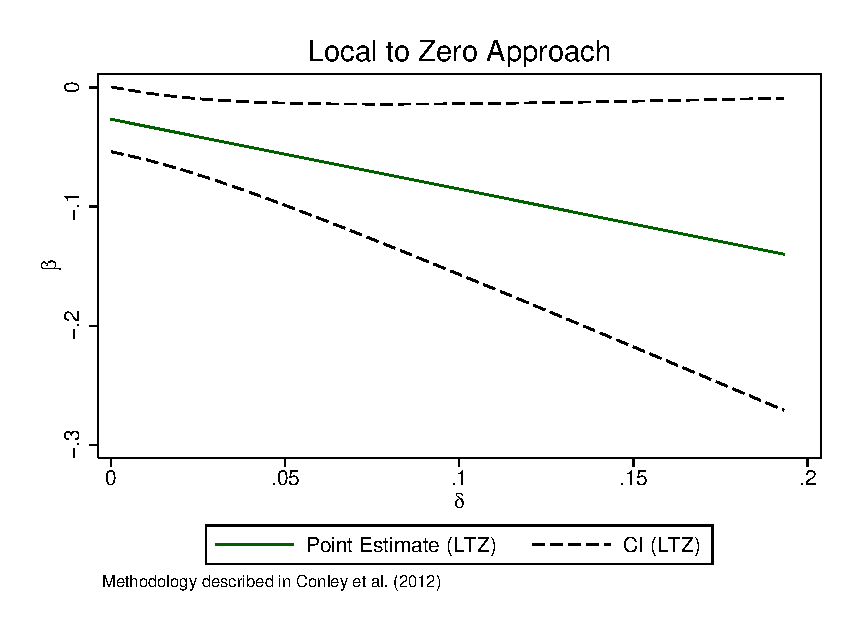
\includegraphics[scale=0.75]{./figures/LTZ_three.eps}
\end{figure}
\hyperlink{two}{\beamergotobutton{2+}}\ \hyperlink{four}{\beamergotobutton{4+}}
\end{frame}

\frame{\frametitle{Bounds: OLS vs.\ IV, Conley et al. }
\begin{itemize}
\item The OLS estimate is $-0.08^{*}$ (parity pooled). 
\begin{itemize}
\item OLS estimates are smaller in absolute terms conditional upon mother characteristics. 
\item Consistent with high fertility women tending to have lower tastes for education.\\ \vspace{5mm}
\end{itemize}
\item First stage indicates twin birth is a powerful instrument. 
\item IV estimates are $-0.04^{*}$ (3+, all) to $-0.06^{*}$ (3+, middle income).
\begin{itemize}
\item IV estimates grow larger in absolute terms conditional upon mother characteristics, consistent with our hypothesis. \\ \vspace{5mm}
\end{itemize}
\item Recognizing that twins are at best plausibly exogenous results in a Q--Q parameter interval with an upper bound of $\sim -0.15$ s.d. \\ \vspace{5mm}
\item Using US data we similarly find a Q--Q tradeoff emerge once we condition upon indicators of maternal health.
\end{itemize}
}

%================================================================================
%== Slide 32: Conclusions
%================================================================================
\section{Conclusions}
\frame{\frametitle{Conclusions}
\begin{itemize}
\item Indicators of mother's health and pregnancy behaviours are significant predictors of twin birth.\\ \vspace{5mm}
\item Conditioning upon available twin predictors produces evidence of a trade-off in IV ($\sim -0.04$ s.d.) and RF estimates.\\ \vspace{5mm}
\item Significantly larger trade-off for middle income countries and for female children\\ \vspace{5mm}
\item Ignoring the twin bias will similarly tend to lead to under-estimation of the trade-off between fertility and women's labour force participation.
\end{itemize}
}

\frame{
\begin{center}
\textcolor{white}{VBP}
\vspace{3cm} \\
{\Large Thank you} 
\vspace{4cm} \\
\footnotesize Source code and data available for inspection: github.com/damiancclarke/twins
\end{center}

}


\section{Appendices}
\frame{
\begin{center}
\Large \textbf{Appendices}
\end{center}
}

\frame{
\begin{center}
\Large \textbf{Appendix Tables}
\end{center}
}

\begin{frame}[label=Fstage]
\frametitle{First Stage: Twins Increase Family Size by $\sim$0.8}
\begin{landscape}\begin{table}[htpb!]\caption{First Stage Results} 
\label{TWINtab:FS}\begin{center}\begin{tabular}{lccccccccc}
\toprule \toprule 
&\multicolumn{3}{c}{2+}&\multicolumn{3}{c}{3+}&\multicolumn{3}{c}{4+}\\ \cmidrule(r){2-4} \cmidrule(r){5-7} \cmidrule(r){8-10} 
\textsc{Fertility}&Base&+S&+S\&H&Base&+S&+S\&H&Base&+S&+S\&H\\ \midrule 
\begin{footnotesize}\end{footnotesize}& 
\begin{footnotesize}\end{footnotesize}& 
\begin{footnotesize}\end{footnotesize}& 
\begin{footnotesize}\end{footnotesize}& 
\begin{footnotesize}\end{footnotesize}& 
\begin{footnotesize}\end{footnotesize}& 
\begin{footnotesize}\end{footnotesize}& 
\begin{footnotesize}\end{footnotesize}& 
\begin{footnotesize}\end{footnotesize}& 
\begin{footnotesize}\end{footnotesize}\\ 
\multicolumn{10}{l}{\textbf{Pre-Twins}}\\ 
Twin&0.798***&0.839***&0.841***&0.796***&0.821***&0.824***&0.841***&0.860***&0.863***\\
&(0.030)&(0.028)&(0.028)&(0.027)&(0.026)&(0.026)&(0.027)&(0.026)&(0.026)\\
\begin{footnotesize}\end{footnotesize}&\begin{footnotesize}\end{footnotesize}&\begin{footnotesize}\end{footnotesize}&\begin{footnotesize}\end{footnotesize}&\begin{footnotesize}\end{footnotesize}&\begin{footnotesize}\end{footnotesize}&\begin{footnotesize}\end{footnotesize}&\begin{footnotesize}\end{footnotesize}&\begin{footnotesize}\end{footnotesize}&\begin{footnotesize}\end{footnotesize}\\\multicolumn{10}{l}{\textbf{Pre-Twins (+bord)}}\\ 
Twin&0.796***&0.838***&0.839***&0.793***&0.825***&0.828***&0.842***&0.863***&0.865***\\
&(0.030)&(0.028)&(0.028)&(0.027)&(0.026)&(0.026)&(0.026)&(0.026)&(0.026)\\
\begin{footnotesize}\end{footnotesize}&\begin{footnotesize}\end{footnotesize}&\begin{footnotesize}\end{footnotesize}&\begin{footnotesize}\end{footnotesize}&\begin{footnotesize}\end{footnotesize}&\begin{footnotesize}\end{footnotesize}&\begin{footnotesize}\end{footnotesize}&\begin{footnotesize}\end{footnotesize}&\begin{footnotesize}\end{footnotesize}&\begin{footnotesize}\end{footnotesize}\\\multicolumn{10}{l}{\textbf{Low-Income}}\\ 
Twin&0.844***&0.861***&0.861***&0.804***&0.822***&0.824***&0.863***&0.866***&0.868***\\
&(0.037)&(0.036)&(0.036)&(0.033)&(0.032)&(0.032)&(0.032)&(0.032)&(0.032)\\
\begin{footnotesize}\end{footnotesize}&\begin{footnotesize}\end{footnotesize}&\begin{footnotesize}\end{footnotesize}&\begin{footnotesize}\end{footnotesize}&\begin{footnotesize}\end{footnotesize}&\begin{footnotesize}\end{footnotesize}&\begin{footnotesize}\end{footnotesize}&\begin{footnotesize}\end{footnotesize}&\begin{footnotesize}\end{footnotesize}&\begin{footnotesize}\end{footnotesize}\\\multicolumn{10}{l}{\textbf{Middle-Income}}\\ 
Twin&0.741***&0.803***&0.806***&0.774***&0.810***&0.815***&0.790***&0.844***&0.846***\\
&(0.051)&(0.045)&(0.045)&(0.047)&(0.044)&(0.044)&(0.047)&(0.043)&(0.043)\\
\begin{footnotesize}\end{footnotesize}&\begin{footnotesize}\end{footnotesize}&\begin{footnotesize}\end{footnotesize}&\begin{footnotesize}\end{footnotesize}&\begin{footnotesize}\end{footnotesize}&\begin{footnotesize}\end{footnotesize}&\begin{footnotesize}\end{footnotesize}&\begin{footnotesize}\end{footnotesize}&\begin{footnotesize}\end{footnotesize}&\begin{footnotesize}\end{footnotesize}\\\multicolumn{10}{l}{\textbf{Desired-Threshold}}\\ 
Twin&0.775***&0.821***&0.822***&0.749***&0.786***&0.788***&0.846***&0.863***&0.865***\\
&(0.036)&(0.033)&(0.033)&(0.030)&(0.029)&(0.029)&(0.028)&(0.028)&(0.028)\\
Twin$\times$desire&0.085&0.064&0.066&0.220***&0.161**&0.165**&-0.031&-0.016&-0.011\\
&(0.067)&(0.062)&(0.062)&(0.070)&(0.066)&(0.066)&(0.085)&(0.079)&(0.080)\\
\begin{footnotesize}\end{footnotesize}&\begin{footnotesize}\end{footnotesize}&\begin{footnotesize}\end{footnotesize}&\begin{footnotesize}\end{footnotesize}&\begin{footnotesize}\end{footnotesize}&\begin{footnotesize}\end{footnotesize}&\begin{footnotesize}\end{footnotesize}&\begin{footnotesize}\end{footnotesize}&\begin{footnotesize}\end{footnotesize}&\begin{footnotesize}\end{footnotesize}\\\multicolumn{10}{l}{\textbf{Twins and Pre-twins}}\\ 
Twin&0.747***&0.801***&0.806***&0.815***&0.831***&0.835***&0.861***&0.863***&0.868***\\
&(0.028)&(0.026)&(0.026)&(0.028)&(0.027)&(0.027)&(0.027)&(0.026)&(0.026)\\
\begin{footnotesize}\end{footnotesize}&\begin{footnotesize}\end{footnotesize}&\begin{footnotesize}\end{footnotesize}&\begin{footnotesize}\end{footnotesize}&\begin{footnotesize}\end{footnotesize}&\begin{footnotesize}\end{footnotesize}&\begin{footnotesize}\end{footnotesize}&\begin{footnotesize}\end{footnotesize}&\begin{footnotesize}\end{footnotesize}&\begin{footnotesize}\end{footnotesize}\\
\midrule\multicolumn{10}{p{18.0cm}}{\begin{footnotesize}\textsc{Notes:} Each cell represents the coefficient from the first-stage of a two-stage regression.  The first-stage represents the effect of twinning at parity $N$ on total fertility where $N$ is 2, 3 or 4 for 2+, 3+ and 4+ groups respectively.  The 2+ group includes all first borns in families with at least 2 births, the 3+ group includes first and second borns in families with at least 3 births, and the 4+ group includes all first to third borns in families with at least four births.  In each regressions the sample is made up of all children aged between 6-18 years from families in the DHS who fulfill these birth order conditions.  Controls in each case are identical to those described in table \ref{TWINtab:IVTwoplus}.  Standard errors are clustered at the level of the mother.$^{*}$p$<$0.1; $^{**}$p$<$0.05; $^{***}$p$<$0.01 
\end{footnotesize}} \\ \bottomrule 
\end{tabular}\end{center}\end{table}\end{landscape}
\hyperlink{FS1}{\beamergotobutton{Back}}
\end{frame}

\begin{frame}[label=Fstage2]
\frametitle{First Stage: Twins Increase Family Size by $\sim$0.8}
\begin{landscape}\begin{table}[htpb!]\caption{First Stage Results} 
\label{TWINtab:FS}\begin{center}\begin{tabular}{lccccccccc}
\toprule \toprule 
&\multicolumn{3}{c}{2+}&\multicolumn{3}{c}{3+}&\multicolumn{3}{c}{4+}\\ \cmidrule(r){2-4} \cmidrule(r){5-7} \cmidrule(r){8-10} 
\textsc{Fertility}&Base&+S&+S\&H&Base&+S&+S\&H&Base&+S&+S\&H\\ \midrule 
\begin{footnotesize}\end{footnotesize}& 
\begin{footnotesize}\end{footnotesize}& 
\begin{footnotesize}\end{footnotesize}& 
\begin{footnotesize}\end{footnotesize}& 
\begin{footnotesize}\end{footnotesize}& 
\begin{footnotesize}\end{footnotesize}& 
\begin{footnotesize}\end{footnotesize}& 
\begin{footnotesize}\end{footnotesize}& 
\begin{footnotesize}\end{footnotesize}& 
\begin{footnotesize}\end{footnotesize}\\ 
\multicolumn{10}{l}{\textbf{Pre-Twins}}\\ 
Twin&0.798***&0.839***&0.841***&0.796***&0.821***&0.824***&0.841***&0.860***&0.863***\\
&(0.030)&(0.028)&(0.028)&(0.027)&(0.026)&(0.026)&(0.027)&(0.026)&(0.026)\\
\begin{footnotesize}\end{footnotesize}&\begin{footnotesize}\end{footnotesize}&\begin{footnotesize}\end{footnotesize}&\begin{footnotesize}\end{footnotesize}&\begin{footnotesize}\end{footnotesize}&\begin{footnotesize}\end{footnotesize}&\begin{footnotesize}\end{footnotesize}&\begin{footnotesize}\end{footnotesize}&\begin{footnotesize}\end{footnotesize}&\begin{footnotesize}\end{footnotesize}\\\multicolumn{10}{l}{\textbf{Pre-Twins (+bord)}}\\ 
Twin&0.796***&0.838***&0.839***&0.793***&0.825***&0.828***&0.842***&0.863***&0.865***\\
&(0.030)&(0.028)&(0.028)&(0.027)&(0.026)&(0.026)&(0.026)&(0.026)&(0.026)\\
\begin{footnotesize}\end{footnotesize}&\begin{footnotesize}\end{footnotesize}&\begin{footnotesize}\end{footnotesize}&\begin{footnotesize}\end{footnotesize}&\begin{footnotesize}\end{footnotesize}&\begin{footnotesize}\end{footnotesize}&\begin{footnotesize}\end{footnotesize}&\begin{footnotesize}\end{footnotesize}&\begin{footnotesize}\end{footnotesize}&\begin{footnotesize}\end{footnotesize}\\\multicolumn{10}{l}{\textbf{Low-Income}}\\ 
Twin&0.844***&0.861***&0.861***&0.804***&0.822***&0.824***&0.863***&0.866***&0.868***\\
&(0.037)&(0.036)&(0.036)&(0.033)&(0.032)&(0.032)&(0.032)&(0.032)&(0.032)\\
\begin{footnotesize}\end{footnotesize}&\begin{footnotesize}\end{footnotesize}&\begin{footnotesize}\end{footnotesize}&\begin{footnotesize}\end{footnotesize}&\begin{footnotesize}\end{footnotesize}&\begin{footnotesize}\end{footnotesize}&\begin{footnotesize}\end{footnotesize}&\begin{footnotesize}\end{footnotesize}&\begin{footnotesize}\end{footnotesize}&\begin{footnotesize}\end{footnotesize}\\\multicolumn{10}{l}{\textbf{Middle-Income}}\\ 
Twin&0.741***&0.803***&0.806***&0.774***&0.810***&0.815***&0.790***&0.844***&0.846***\\
&(0.051)&(0.045)&(0.045)&(0.047)&(0.044)&(0.044)&(0.047)&(0.043)&(0.043)\\
\begin{footnotesize}\end{footnotesize}&\begin{footnotesize}\end{footnotesize}&\begin{footnotesize}\end{footnotesize}&\begin{footnotesize}\end{footnotesize}&\begin{footnotesize}\end{footnotesize}&\begin{footnotesize}\end{footnotesize}&\begin{footnotesize}\end{footnotesize}&\begin{footnotesize}\end{footnotesize}&\begin{footnotesize}\end{footnotesize}&\begin{footnotesize}\end{footnotesize}\\\multicolumn{10}{l}{\textbf{Desired-Threshold}}\\ 
Twin&0.775***&0.821***&0.822***&0.749***&0.786***&0.788***&0.846***&0.863***&0.865***\\
&(0.036)&(0.033)&(0.033)&(0.030)&(0.029)&(0.029)&(0.028)&(0.028)&(0.028)\\
Twin$\times$desire&0.085&0.064&0.066&0.220***&0.161**&0.165**&-0.031&-0.016&-0.011\\
&(0.067)&(0.062)&(0.062)&(0.070)&(0.066)&(0.066)&(0.085)&(0.079)&(0.080)\\
\begin{footnotesize}\end{footnotesize}&\begin{footnotesize}\end{footnotesize}&\begin{footnotesize}\end{footnotesize}&\begin{footnotesize}\end{footnotesize}&\begin{footnotesize}\end{footnotesize}&\begin{footnotesize}\end{footnotesize}&\begin{footnotesize}\end{footnotesize}&\begin{footnotesize}\end{footnotesize}&\begin{footnotesize}\end{footnotesize}&\begin{footnotesize}\end{footnotesize}\\\multicolumn{10}{l}{\textbf{Twins and Pre-twins}}\\ 
Twin&0.747***&0.801***&0.806***&0.815***&0.831***&0.835***&0.861***&0.863***&0.868***\\
&(0.028)&(0.026)&(0.026)&(0.028)&(0.027)&(0.027)&(0.027)&(0.026)&(0.026)\\
\begin{footnotesize}\end{footnotesize}&\begin{footnotesize}\end{footnotesize}&\begin{footnotesize}\end{footnotesize}&\begin{footnotesize}\end{footnotesize}&\begin{footnotesize}\end{footnotesize}&\begin{footnotesize}\end{footnotesize}&\begin{footnotesize}\end{footnotesize}&\begin{footnotesize}\end{footnotesize}&\begin{footnotesize}\end{footnotesize}&\begin{footnotesize}\end{footnotesize}\\
\midrule\multicolumn{10}{p{18.0cm}}{\begin{footnotesize}\textsc{Notes:} Each cell represents the coefficient from the first-stage of a two-stage regression.  The first-stage represents the effect of twinning at parity $N$ on total fertility where $N$ is 2, 3 or 4 for 2+, 3+ and 4+ groups respectively.  The 2+ group includes all first borns in families with at least 2 births, the 3+ group includes first and second borns in families with at least 3 births, and the 4+ group includes all first to third borns in families with at least four births.  In each regressions the sample is made up of all children aged between 6-18 years from families in the DHS who fulfill these birth order conditions.  Controls in each case are identical to those described in table \ref{TWINtab:IVTwoplus}.  Standard errors are clustered at the level of the mother.$^{*}$p$<$0.1; $^{**}$p$<$0.05; $^{***}$p$<$0.01 
\end{footnotesize}} \\ \bottomrule 
\end{tabular}\end{center}\end{table}\end{landscape}
\hyperlink{IV}{\beamergotobutton{Back}}
\end{frame}

\begin{frame}[label=sumStatsN]
\input{./tables/NHISstats.tex}
\hyperlink{sumStats}{\beamergotobutton{Back}}
\end{frame}


 \begin{frame}[label=Spain1]
\begin{table}
\caption{Probability of Twin Birth: Spain Administrative Data 2007--2012}
\begin{center}
\scalebox{0.6}{
\begin{tabular}{lc}
\hline
VARIABLES	&	Twin*100 \\	\hline
	&	(1)	\\
Primary Education (Mother)	&	  -.04713**	\\
	&	 (0.02404)	\\
      Secondary Education (Mother)	&	  -.11682***	\\
	&	(0.02528)	\\
   Tertiary Education (Mother)	&	  -.03166	\\
	&	(0.02766)	\\
  Parents are Immigrants	&	  -.17078***	\\
	&	(0.03354)	\\
        citm	&	   .38144***	\\
	&	(0.03247)	\\
 Married	&	   .63864***	\\
	&	(0.01844)	\\
    Mother's Age	&	   1.63192***	\\
	&	(0.09688)	\\
    Mother's Age$^2$	&	  -.05818***	\\
	&	(0.00342)	\\
   Father's Age	&	  -.17344***	\\
	&	(0.04788)	\\
   Father's Age$^2$	&	   .00621***	\\
	&	(0.00137)	\\
   No Father	&	  -.48331	\\
	&	(0.53907)	\\
    Constant	&	  -13.20683	\\
	&	(0.94074)	\\
	& \\
	Observations & 2,869,329 \\
	$R^2$ & 0.0068 \\ \hline
\end{tabular}}
\end{center}
\end{table}

\hyperlink{c}{\beamergotobutton{Back}}
\end{frame}

 \begin{frame}[label=Brazil]
\begin{table}[htpb!]
\caption{Probability of Twin Births: Brazil Administrative Data}
\begin{center}
\scalebox{0.56}{

\begin{tabular}{llcc}\hline

&&(1)&(2)\\ \cmidrule(r){3-4}
&&\multicolumn{2}{c}{Probability for twin}\\ \hline
&&&\\

Female	&		&	0.0012***	&	0.0012***	\\
	&		&	(0.0001)	&	(0.0001)	\\
Age	&		&	0.0008***	&	0.0009***	\\
	&		&	(0.0000)	&	(0.0000)	\\
Marital status	&	Married	&	0.0008***	&	0.0009***	\\
	&		&	(0.0001)	&	(0.0001)	\\
	&	Divorced	&	0.0002	&	0.0002	\\
	&		&	(0.0006)	&	(0.0006)	\\
Years of schooling	&		&	-0.0000**	&	-0.0000**	\\
	&		&	(0.0000)	&	(0.0000)	\\
Number of live births&	&		0.0006***	&	0.0005***	\\
	&		&	(0.0000)	&	(0.0000)	\\
Number of still births&		&	-0.0001**	&	-0.0002***	\\
	&		&	(0.0001)	&	(0.0001)	\\
Race	&	Black	&	-0.0011***	&	-0.0014***	\\
	&		&	(0.0002)	&	(0.0002)	\\
	&	Asian	&	-0.0014***	&	-0.0019***	\\
	&		&	(0.0005)	&	(0.0005)	\\
	&	Mixed	&	-0.0016***	&	-0.0019***	\\
	&		&	(0.0001)	&	(0.0001)	\\
	&	Indigenous	&	-0.0057***	&	-0.0065***	\\
	&		&	(0.0004)	&	(0.0004)	\\
Number of prenatal visits	&		&		&	-0.0005***	\\
	&		&		&	(0.0000)	\\
Constant	&		&	-0.0035***	&	-0.0009***	\\
	&		&	(0.0001)	&	(0.0002)	\\
R-squared	&		&	0.0020	&	0.0021	\\ \hline
\multicolumn{4}{p{12cm}}{\begin{footnotesize}Notes: Standard errors are clustered at the municipality level. Number of observations = 20,013,814. *** $p<0.01$, ** $p<0.05$, * $p<0.1$ \end{footnotesize}}\\




\end{tabular}}


\end{center}
\end{table}

\hyperlink{c}{\beamergotobutton{Back}}
\end{frame}

\begin{frame}[label=UK]
 \begin{table}[htpb!] 
\caption{Probability of Giving Birth to Twins (UK)} 
\label{TWINtab:UK} 
\begin{center}
\scalebox{0.6}{
\begin{tabular}{lclc} \toprule \toprule 
&(1)&&\\
Twin$\times$100&&&\\\midrule
\midrule\multicolumn{4}{p{11cm}}{\begin{footnotesize}\textsc{Notes:}$^{*}$p$<$0.1; $^{**}$p$<$0.05; $^{***}$p$<$0.01\end{footnotesize}}\\ \hline \normalsize \end{tabular}}\end{center}\end{table}

\hyperlink{c}{\beamergotobutton{Back}}
\end{frame}

\begin{frame}[label=Spain3]
\begin{table}
\caption{Twins, Miscarriage and Maternal Health (Administrative Data from Spain)}
\begin{center}
\scalebox{0.76}{
\begin{tabular}{lclc}
\hline 
VARIABLES	&	Fetal Death$	\times$100 & & \\	\hline
	&	(1) & &	\\
Primary	&	  -0.60179*** &	Primary$	\times$Twin	&	   -0.6618***	\\
	&	 (0.01456)	& &	 (0.20926)	\\
Secondary	&	  -0.71998*	& Secondary$	\times$Twin	&	  -0.55901***	\\
	&	  (0.0151)	& 	&	 .0020978	\\
Tertiary	&	  -0.80019***	& Tertiary$	\times$Twin	&	  -0.65091***	\\
	&	(0.01582)	& 	&	(0.20866)	\\
Immigration	&	  -0.07223***	& Immigration$	\times$Twin	&	  0.22871	\\
	&	 (0.0171)	& 	&	(0.29614)	\\
City	&	  -0.00321	& City$	\times$Twin	&	  0.09566	\\
	&	(0.01584)	& 	&	 (0.26876)	\\
Married	&	  -0.07354***	&Married$	\times$Twin	&	  -0.08978	\\
	&	 (0.00759)	&	&	 (0.11893)	\\
No Father	&	0.68626***	&No Father$	\times$Twin	&	3.25232	\\
	&	 (0.23825)	&	&	(4.09309)	\\
Constant	&	-1.35966***	& & \\
	&	(0.33674)	& &  \\
	& \\
	Obs & 2,869,329 & & \\
	$R^2$ & 0.0044  & & \\ \midrule
	\multicolumn{4}{p{8cm}}{Note: Spanish administrative births: 2007-2012.}
\end{tabular}}
\end{center}
\end{table}

\hyperlink{mechan}{\beamergotobutton{Back}}
\end{frame}

\begin{frame}[label=USA3]
\input{./tables/USfdeaths1.tex}
\end{frame}

\begin{frame}
\input{./tables/USfdeaths2.tex}
\end{frame}

\begin{frame}
\input{./tables/USfdeaths3.tex}
\hyperlink{mechan}{\beamergotobutton{Back}}
\end{frame}


\begin{frame}[label=MMRselec]
\frametitle{Height and Selective Maternal Survival (1)} 
\begin{itemize}
\item We use unique data on maternal mortality rates of sisters of female respondents in the DHS.
\item We count the number of `unhealthy' women whose sisters died ($N_u$) and the number of `healthy' women whose sisters died ($N_h$).
\item We assume $N_u > N_h$ given that our \hyperlink{MMRcuts}{\textcolor{blue}{data show}} that maternal mortality (of sisters) depends upon height (assumes height correlated across sisters).
\item First, we expand our sample to include $N_u + N_h$ women, choosing them randomly from within our file, based upon their `health'.
\item We use different measures of `health' to check sensitivity of results to this. We use different thresholds and combine being short and being underweight.
\end{itemize}
\end{frame}

\begin{frame}
\frametitle{Height and Selective Maternal Survival (2)}
\begin{itemize}
\item Second, we assume that the unhealthy women who died in childbirth were all carrying twins and that the healthy women who died in childbirth were all carrying singletons. 
\item This is an extreme assumption intended to produce a severe test of selection.
\item We then re-estimate the regression of prob(twin) on indicators of mother's health using the simulated sample.
\item We continue to find significant impacts of maternal health on twinning probabilities. So selection is not driving our results.
\end{itemize}
\end{frame}
	

\begin{frame}[label=surv]
\input{./tables/Alderman.tex}
\hyperlink{robust}{\beamergotobutton{Back}}
\end{frame}

\frame{
\begin{center}
\Large \textbf{Appendix Figures}
\end{center}
}

\frame{\frametitle{Twins Are More Likely to Occur at Higher Birth Orders}
\begin{figure}[htpb!]
\centering
  %\caption{Total births by Family Type}
  %\label{TWINfig:famsize}
  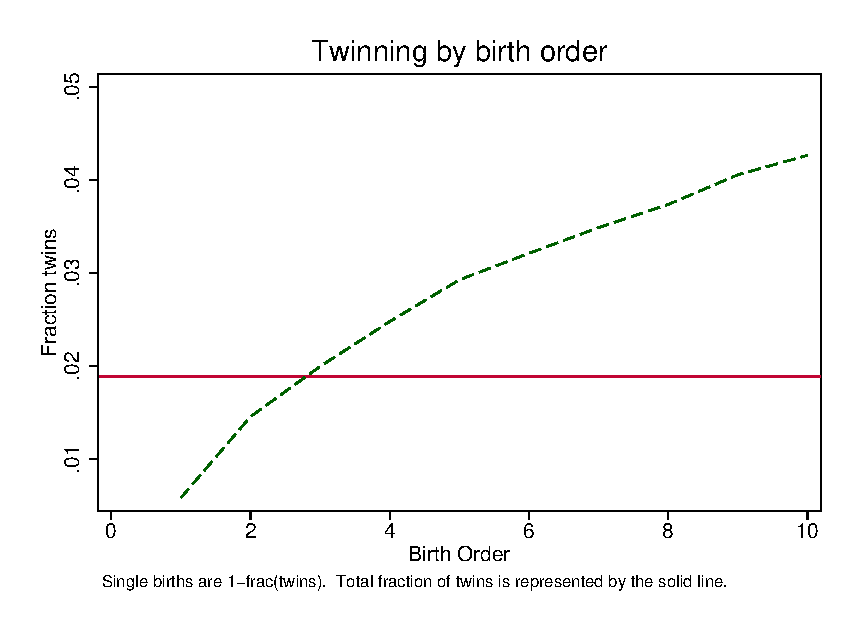
\includegraphics[scale=0.75]{./figures/twinbybord.eps}
\end{figure}
}

\begin{frame}[label=MMRcuts]
\frametitle{Height and Selective Survival}
\begin{figure}[htpb!]
\centering
  \includegraphics[scale=0.75]{./figures/MMRcuts.eps}
\end{figure}
\hyperlink{MMRselec}{\beamergotobutton{Back}}
\end{frame}


\begin{frame}[label=two]
\frametitle{Estimates (2+) Assuming that $\gamma \sim U(0,\delta)$}
\begin{figure}[htpb!]
\centering
  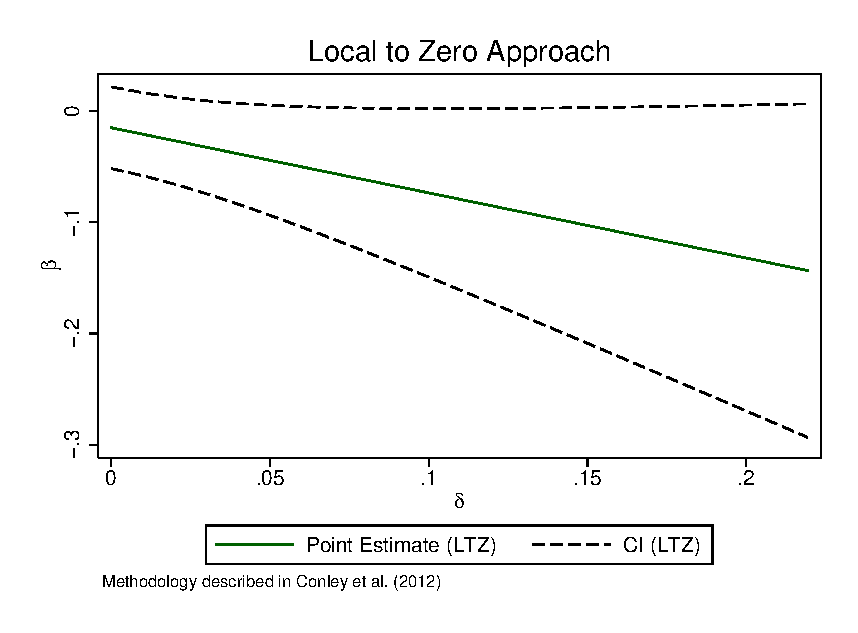
\includegraphics[scale=0.75]{./figures/LTZ_two.eps}
\end{figure}
\hyperlink{Conley3}{\beamergotobutton{Back}}
\end{frame}

\begin{frame}[label=four]
\frametitle{Estimates (4+) Assuming that $\gamma \sim U(0,\delta)$}
\begin{figure}[htpb!]
\centering
  \includegraphics[scale=0.75]{./figures/LTZ_four.eps}
\end{figure}
\hyperlink{Conley3}{\beamergotobutton{Back}}
\end{frame}

\begin{frame}[label=gammaResamp]
\frametitle{Bootstrap Estimates of $\hat\gamma$}
\begin{figure}[htpb!]
\centering
  \includegraphics[scale=0.7]{./figures/gammaResamp.eps}
\end{figure}
\hyperlink{gammaDiscuss}{\beamergotobutton{Back}}
\end{frame}

\end{document}

%********************************************************************************
%********************************************************************************
%********************************************************************************
%********************************************************************************
%********************************************************************************
%********************************************************************************
%********************************************************************************
%********************************************************************************
%********************************************************************************
%********************************************************************************
